% Original real d=1,r=2 model: range(B) is a line in the two-coordinate record space.
\documentclass[tikz,border=4mm]{standalone}
\usepackage{amsmath}
\begin{document}
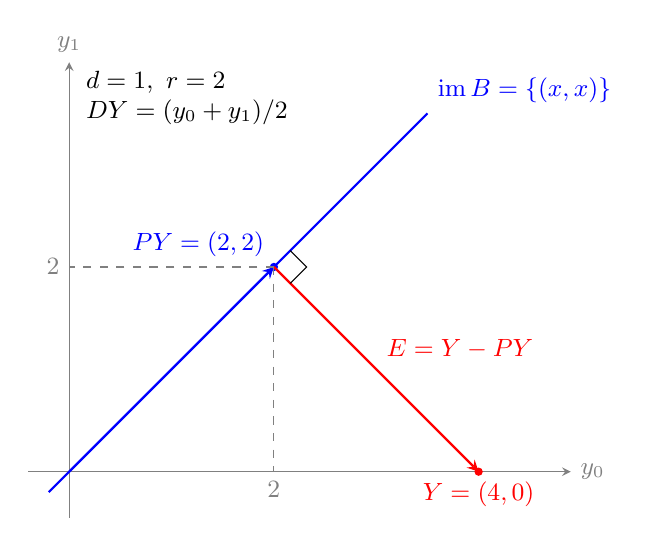
\begin{tikzpicture}[>=stealth,font=\small,x=1.3cm,y=1.3cm]
\draw[->,gray] (-.4,0)--(4.9,0) node[right] {$y_0$};
\draw[->,gray] (0,-.45)--(0,4) node[above] {$y_1$};
\draw[blue,thick] (-.2,-.2)--(3.5,3.5) node[above right] {$\operatorname{im}B=\{(x,x)\}$};
\draw[->,blue,thick] (0,0)--(2,2);
\fill[blue] (2,2) circle (1.5pt) node[above left] {$PY=(2,2)$};
\fill[red] (4,0) circle (1.5pt) node[below] {$Y=(4,0)$};
\draw[->,red,thick] (2,2)--(4,0) node[midway,above right] {$E=Y-PY$};
\draw[dashed,gray] (2,2)--(2,0) node[below] {$2$};
\draw[dashed,gray] (2,2)--(0,2) node[left] {$2$};
\draw (2.16,2.16)--(2.32,2)--(2.16,1.84);
\node[align=left] at (1.15,3.65) {$d=1,\ r=2$\\$DY=(y_0+y_1)/2$};
\end{tikzpicture}
\end{document}
